\section{Method}

\subsection{Data preprocessing}
Bla.

\subsection{Text vectorization}
\subsubsection{Textvectorizer}

The first set of vectorizers focuses on the texts of the documents. The \emph{textvectorizer} is a very generic approach that can be used on any corpus of textual documents. In the StarFish context, we define 'content' as the title and text-fields of a document. The only exception on this are Persons, of which we wil use the name and about-fields. 

The textvectorizer first transforms the set of documents into a bag of words and calculates the TF-IDF values for all words. This was done using the TFIDFVectorizer of scikitlearn \citep{scikit-learn}.  Though the TF-IDF values of words that are used very often should be low, common words such as 'and', 'or' and 'of' are still present in the vectors. This could be caused by the different types of documents. For example, a Question often structured in a less complex way than a Project description. To prevent this from happening, the English stopword list that comes standard with scikit learn was used to remove these words from the document descriptors.

\subsubsection{Weighted textvectorizer}
The weighted text vectorizer is an extension of the textvectorizer that takes into account the links of the proposed documents. The vectors of the links of a document are added with some weight to the vectors of the documents themselves. Intuitively, this would add semantic information about a document based on it's links. For example, a Person is likely to write other documents about his or her subjects of expertise. Knowing not only the biography of a Person, but also the content he or she has added to Starfish, gives a more complete image of what documents could be related to that Person.

The vectors of links of a document are added in a recursive way, where documents that are linked directly have a higher weight than documents that are linked transitively. The algorithm is displayed in figure xx.

\subsection{Tag vectorization}
\subsubsection{Simple tag vectorizer}
The tag-based approach is more StarFish specific than the text-based approach, since it depends on the tags that are available in StarFish. The tags on StarFish are added by the users themselves, so offer a human-based vision on what a document is really about. The simple tag vectorizer is a very straight forward implementation of the idea of using tags. The vectors of this transformation consist of a binary list that tells whether or not a tag is attached to the document. 

\subsubsection{Tag smoothing}
The tag smoothing vectorizers creates descriptors based on the tag set of a document. A tag co-occurs with other tags in a document, we assume documents with similar tags should be linked in Starfish. Let the frequency of occurrence with other tags across the dataset will form a vector for each tag. The descriptor for a document is then created by combining the occurrence vectors for all the document's tags. Now documents with tags that occur together will be seen as similar.

There are two reasons why one would like to smooth the tag co-occurences. Firstly, a problem for this is that tags must occur together before the algorithms works properly. The Starfish dataset contains a lot of tags that only occur with a small frequency, which means the tag occurrence vector will contain many zeros. This makes the algorithm perform bad with little data. Secondly, two tags can describe the same concept and be connected to that concept through a common co-occurence with another tag. Whilst they describe the same concept and are connected to that, they are not directly linked together. Therefore it seems feasible to perform some sort of smoothing on the co-occurences of tags.

\citet{zhou2011web} proposed a method to cluster web documents based on tag set similarity. This is based on a similarity between two tags as a relation between the frequency these tags occur separate and together, as described in equation~\ref{eq:tag_similarity}. To smooth these similarities between tags, a tag similarity matrix $\mathcal{C}$ is constructed. Each entry $c_{i,j}$ in this matrix can be viewed as the angle $\theta_{i,j}$ between two unknown vectors $v_i$ and $v_j$. These vectors cover both explicit similarity and implicit similarity \citep{park2010vector}. This transfers the problem to find a set of linearly independent vectors $\{v_1,v_2,\ldots,v_n\}$ for which for all $v_i \cdot v_j = \cos(\theta_{i,j})$. One must find a matrix $\mathcal{V}$ for which $V^TV = C$. This can be done by orthogonal triangularization on $\mathcal{C}$ for which \citeauthor{zhou2011web} introduces a modified Cholesky transform.

\begin{equation} \label{eq:tag_similarity}
s_{i,j} = \frac{f_{i,j}}{f_i + f_j - f_{i,j}}
\end{equation}


\subsubsection{Glossaries of tags}
\begin{itemize}
\item Motivation: find underlying network between tags by using their glossaries
\item Implementation: hybrid form of text and tag vectorizer
\end{itemize}

\subsection{Distance metrics}
Short description of how these were implemented

\subsection{Bayesian weighting}
Explain motivation, theory and implementation 

\subsection{Thresholds}
In figure~\ref{fig:thresholds} the distances for nearby documents we recommend can be viewed. It is clear that different vecotrizers return different curves of increase of distance. The lines for documents with zero links do not seem to follow a specific pattern, the lines for documents with more links are better clustered. 


\begin{figure}[h]
\subfigure[Weighted tags]{	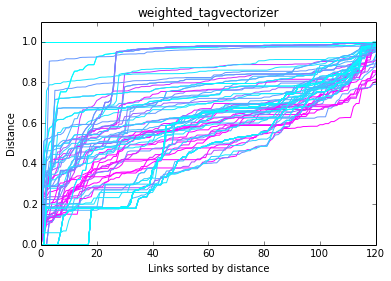
\includegraphics[width =0.45\textwidth]{images/threshold_weighted_tag} }
\subfigure[text]{	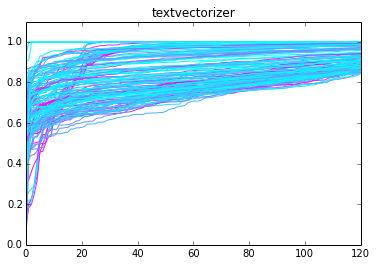
\includegraphics[width =0.45\textwidth]{images/threshold_text} }
\subfigure[tag smoothing]{	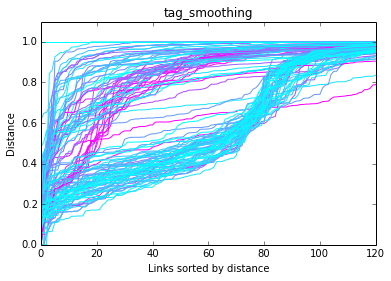
\includegraphics[width =0.45\textwidth]{images/threshold_smoothing} }
\subfigure[glossaries]{	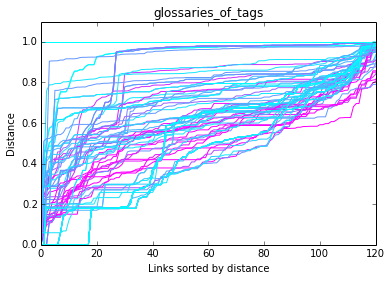
\includegraphics[width =0.45\textwidth]{images/threshold_glossary} }
\caption{The blue purple gradient represents documents with 0 links (blue) to >10 links (purple)}
\label{fig:thresholds}
\end{figure}

Explan motivation, theory and implementation